\chapter{Konzeption des Frameworks}
\label{chap:konzeption_pubsub}
In diesem Kapitel wird die Konzeption des Frameworks zur Verteilungsoptimierung in seinen Einzelheiten erläutert. Ausgehend von den in \cite{Ficher2010a} identifizierten Eventtypen und Optimierungsdimensionen wird im nächsten Abschnitt beschriebene Problemstellung greifbar. Das Framework muss generisch auf vielfältige Weisen anpassbar sein ohne teure Laufzeiteinbußen zu bedingen \cite{NEW_PAPER} \missing{CITE: NEW PAPER!}. Weiterhin darf die Konzeption, \ac{m2etis} als ein einfach zu nutzendes kanalbasiertes Publish/Subscribe-System zu darzustellen nicht aus dem Fokus geraten. Die Problemstellung führt zum Verarbeitungsmodell das beispielhaft getestet wird.

Im Optimierungsschritt erzeugt \ac{m2etis} für jeden Eventtypen einen optimierten Kanal der über das Publish/Subscribe-System ansprechbar ist. Dieses bieten die bekannten Methoden \emph{subscribe, unsubscribe} und \emph{publish} an. Jeder Kanal ist entlang den Dimensionen derart optimiert, dass Nachrichten des Eventtypen bestmöglich verarbeitet und über Netzwerk verteilt werden können. Das Netzwerk selbst wird über die \ac{kbr}-API angesprochen, die ihrerseits drei Methoden anbietet um den Nutzer über Ein- und austritte von Knoten sowie über den Knoten zu routende und auch ankommende Nachrichten zu informieren \cite{Dabek2003Towards} (siehe auch \Fref{chap:evaluation_p2p:generic_api}). Damit ein Kanal nur jene Nachrichten bearbeitet die für ihn bestimmt sind, werden eigene Nachrichtentypen am Netzwerk registriert.

Für die logische Umsetzung der in \cite{Fischer2010Event} identifizierten semantischen Dimensionen eines Eventtypen wird der Begriff \emph{Policy} eingeführt. Eine Policy definiert dabei Schnittstelle für verschiedene konkrete Implementierung (genannt Strategie) und deren Auswirkung auf die Nachrichtenverarbeitung im Publish/Subscribe-System. Die folgenden sieben Policies decken die Dimensionen ab \cite{NEW_PAPER}.\missing{CITE: NEW PAPER!}

\begin{description}
\item[Verteilung] bestimmt die Verteilung der Events und den Aufbau des Multicast-Trees, mittels dem die Nachrichten versandt werden \cite{KostasKatrinis2005}.
\item[Filterung] erlaubt es Anmeldungen Prädikate mitzugeben. Es stellt sicher, dass diese Prädikate nach oben im Multicast-Tree zusammengeführt werden, damit Nachrichten frühzeitig gefiltert werden können. Dies bedeutet, dass Nachrichten jeweils beim logischen Absender gefiltert werden müssen.
\item[Zustellung] bestimmt das Kommunikationspradigma des Nachrichtenversand und leitet z.B. Bestätigungen über eingegangene Nachrichten an den sendenden Knoten ein.
\item[Reihenfolge] definiert die Synchronisationskonzept der Nachrichten in einem Kanal.
\item[Persistenz] bietet die Möglichkeit an verschickte Nachrichten zu speichern.
\item[Sicherheit] gibt eine Schnittstelle zur Nachrichtenverschlüsselung vor.
\item[Validität] prüft die ankommenden Nachrichten auf ihre Validität. Frühzeitig verworfene Nachrichten können das Nachrichtenaufkommen im System stark vermindern.
\end{description}

Die Verbindung der Publish/Subscribe Methoden und der genutzten \ac{kbr} Methoden ist trivial, da jede verschickte Nachricht durch die Methoden \emph{forward} und \emph{deliver} des Netzwerkes verarbeitet wird \cite{Dabek2003Towards}.\\
Die Verteilung der Policies auf die verschiedenen Nachrichtentypen ist hingegen interessanter und in \Fref{tab:verbindungsmatrix} aufgezeigt. Bei der Verarbeitung von \emph{Publish}-Nachrichten, den eigentlichen Events, wird jede Policy abgefragt. Die \emph{Subscribe}- und \emph{Unsubscribe}-Nachrichten dienen jedoch nur zum Aufbau und der Verwaltung des Multicast-Treesrm. Aus diesem Grund werden bei diesen Nachrichtentypen nur die Policies Verteilung, Filterung und Sicherheit gebraucht.

\begin{table}[!h]
\resizebox{\textwidth}{!}{%
\begin{tabular}{llccccccc}
\toprule
Nachrichten- & KBR	& \multicolumn{7}{c}{Policy pro Kanal} \\
\cmidrule{3-9}
typ				&	Methode	& Verteilung & Filterung & Zustellung & Reihenfolge & Persistenz & Sicherheit & Validität \\
\midrule
publish	    & deliver & + & + & + & + & + & + & + \\
\midrule
subscribe	  & deliver & + & + &   &   &   & + & \\
\cmidrule{2-9}
			      & forward & + & + &   &   &   & + & \\
\midrule
unsubscribe & deliver & + & + &   &   &   & + & \\
\cmidrule{2-9}
      & forward & + & + &   &   &   & + & \\
\bottomrule
\end{tabular}}
\caption{Verbindungsmatrix}
\label{tab:verbindungsmatrix}
\end{table}

Events, also Publish-Nachrichten, werden ausschließlich in deliver behandelt, so dass diese bei allen Empfängern ankommen und unterwegs nicht verändert oder terminiert werden können. Dies ist ein kleiner Schritt in die Richtung zur Betrugsverhinderung. Für Subscribe- und Unsubscribe-Nachrichten entscheidet die eingesetzte Verteilungsstrategie darüber, ob diese in forward und/oder deliver behandelt werden. Nur in foward haben die beiden Strategien Verteilung und Filter die Möglichkeit die zu weiterleitende Nachricht zu verändern oder gar zu terminieren. Dies bedeutet, dass jede Filterstrategie generisch beide Varianten unterstützen muss.


\section{Verarbeitungsmodell}
Based on the given mapping, the challenge is to find a generic application order for the policies in the processing model.
Die richtige Reihenfolge der Policies bei der Verarbeitung der Nachrichten ist bestimmend für eine gute Blupp.

Beim Erstellen einer Nachricht, werden Verwaltungsinformationen der einzelnen Policies abgefragt und mit der Nachricht verschickt. Anhand dieser Informationen kann die Nachricht auf einem anderen Knoten entsprechend behandelt werden. Subscribe- und Unsubscribenachrichten bestehen nur aus diesen Verwaltungsinformationen, da sie zum Aufbau und der Verwaltung des Multicast-Trees dienen und keine Events transportieren.

Der Versand einer Nachricht ist in \Fref{fig:processing_send} bildlich dargestellt. Nachdem die Nachricht erstellt ist, wird die Verteilungspolicy nach einer Liste von Empfängern befragt. Diese ist vom Nachrichtentyp abhängig. Für Subscribe- und Unsubscribenachrichten ist dies immer Rootknoten des Multicast-Trees, da dieser dessen Aufbau koordiniert, beziehungsweise dies durch die Knoten auf dem Routingpfad durch das Netzwerk geschieht. Ist es eine Publish-Nachricht, so ist der Empfänger der Rootknoten, falls die Nachricht mit \emph{to root} gekennzeichnet ist. Dies ist der Fall, wenn ein Knoten einen Event in das System bringen möchte. Jeder Event muss an den/die Rootknoten geschickt werden, da die Verteilung innerhalb der Methode deliver stattfindet. Hat die Nachricht den/die Rootknoten erreicht, so ist sie mit \emph{from root} gekennzeichnet und die Verteilungsstrategie gibt als Empfänger die eingeschriebenen Knoten aus. Für jeden Eintrag dieser Liste wird nun von der Filterstrategie geprüft, ob die Nachricht auf das mit diesem Knoten verbundene Prädikat passt. Hiermit kann die Anzahl der zu versendenden Nachrichten reduziert werden. Schließlich wird die Nachricht durch die anhand der Sicherheitsstrategie vorgegebene Verschlüsselung kodiert und über das Netzwerk an alle Empfänger gesandt.

\begin{figure}[htbp]
\centering
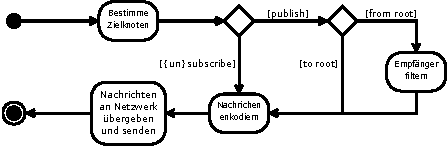
\includegraphics{grafics/processing_send.pdf}
\caption{Verarbeitungsmodell}
\label{fig:processing_send}
\end{figure}

Sollten Nachrichten in forward behandelt werden, so werden diese zuerst dekodiert wie es in \Fref{fig:processing_forward} aufgezeigt ist. Die Verteilungs- und Filterpolicies können anhand der Verwaltungsinformationen ihren Zustand anpassen und wenn nötig die Nachricht ändern oder gar stoppen.

\begin{figure}[htbp]
\centering

\includegraphics{grafics/processing_forward.pdf}
\caption{Verarbeitungsmodell}
\label{fig:processing_forward}
\end{figure}

Die Abarbeitung der Nachrichten in deliver ist komplexer als die beiden oben genannten Fälle, da hier alle Policies zusammenarbeiten wie es \Fref{fig:processing_deliver} aufzeigt. Nach der Entschlüsselung werden Subscribe- und Unsubscribenachrichten ähnlich wie bei der Behandlung in forward verarbeitet. Die Policies können ihren Zustnad aktualisieren.\\
Publishnachrichten müssen eine Validitätsprüfung bestehen, bevor entschieden wird, ob sie eine Nachricht \emph{to root}, also an den Rootknoten sind, oder nicht. Der Rootknoten und alle andern Knoten auf dem Verteilungsweg, die selbst Verteilungsaufgaben übernehmen müssen (abhängig von der gewählten Verteilungsstrategie), leiten nun das Verteilen der Nachricht ein. Dazu wird in einem ersten Schritt eine neue Publishnachricht erstellt, alle Verwaltungsinformationen abgefragt und schließlich die Nachricht mit dem obig beschriebenen Verfahren gesendet. Nun wird an diesen Knoten geprüft ob sie selbst angemeldet sind und ob sie in diesem Falle an der Nachricht interessiert sind. Wenn nein, so endet die Bearbeitung. Ansonsten trifft sich der Ablaufpfad an dieser Stelle mit dem Ablaufpfad einfacher Knoten, die lediglich Subscriber sind. Die Synchronisierungspolicy ermöglicht eine Wohlordnung der Nachricht und kann diese sowohl zurückhalten als auch mehrer Nachrichten zurückgeben. Diese Nachrichten werden nun nochmals auf ihre Validität geprüft, da zurückgehaltene Nachrichten inzwischen veraltet sein können. Für jede valide Nachricht wird eine Signalisierung der Zustellung laut Policy, z.B. eine Acknowledgementnachricht zurück an den Sender, ermöglicht. Bevor eine Nachricht an die Applikation übergeben wird, kann sie persistiert werden.

\begin{figure}[htbp]
\centering
\resizebox{\textwidth}{!}{%
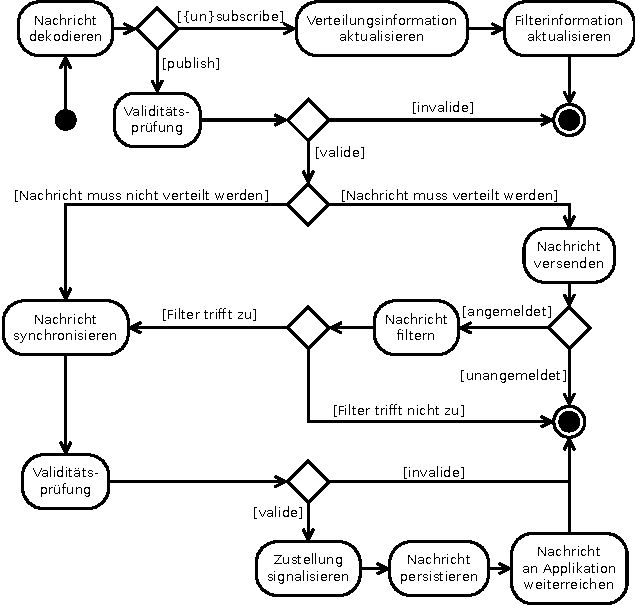
\includegraphics{grafics/processing_deliver.pdf}}
\caption{Verarbeitungsmodell}
\label{fig:processing_deliver}
\end{figure}


\subsection{Beispielhafte Strategien}
For every policy \ac{m2etis} provides one ore more implementations. For example \emph{Direct} or \emph{Multicast} for routing. The framwork permits inclusion of more user-defined strategies. Different types of channel use a different set of implementations for every policy, creating a variety of optimization options. Each implemented strategy must provide additional cost information that is used in the optimizing step and they may add information onto each message to enable the customized treatment.

Using the example of Scribe \cite{Castro2002Scribe} and VON \cite{Hu2006VON} some details and inner workings of the processing model showed in figure \ref{fig:deliver} are explained. Scribe creates a multicast-tree trying to minimize the amount of messages while an algorithm like VON is neighborhood centric.

Using a scribe-like algorithm for routing \emph{Get Targetnodes} returns either the calculated root node for the channel or the list of subscribed nodes to which a publication must be forwarded. On the other hand a routing strategy like VON returns the in-game neighbors, obtained through application-level knowledge, as each node subscribes at his neighbors in the virtual world. Publications are sent to self enabling the distribution in deliver.

Scribe processes unsubscribe and subscribe messages in forward. Each node on the routing path adds the sender to its list of subscribers and can changes the message to create the multicast-tree. The periodic resubscription is triggerd externally for subscribed nodes as the channel will call its own subscribe method again or internally for intermediate routing hops as the algorithm will resend its subscriptions if other nodes down in the multicast-tree will refresh their subscribtion. It is necessary that the filter strategy is always involved to ensure the correct merge of predicates upwards the logical mulitcast-tree.

VON on the other hand does not need automatic periodic subscriptions, because each node will unsubscribe and subscribe frequently. Using the example of position updates it is obvious that each node and its neighbors move often and need to alter their subscribtions each frame in the game.

Using TTL or a timestamp-based approach for the strategy implementing the validity policy, the TTL would be increased on every routing hop or the passed time since the message was created is tested against the interval set in the strategy.

This exemplary discussion of different strategies indicates the generic nature of our processing model in terms of a multidimensional optimization for publish/subscribe channels.
